\documentclass{report}

\usepackage{amsmath}
\usepackage{amssymb}	
\usepackage{graphicx}
\usepackage{float}
\newcommand{\HRule}{\rule{\linewidth}{0.5mm}}
\setlength{\parindent}{0in}
\setlength{\parskip}{12pt}
\usepackage[margin=0.8in]{geometry}
\usepackage{algorithm}
\usepackage{algpseudocode}

\usepackage{listings}
\usepackage{xcolor}
\lstset { %
    language=C++,
    backgroundcolor=\color{black!5}, % set backgroundcolor
    basicstyle=\footnotesize,% basic font setting
}

\definecolor{codegreen}{rgb}{0,0.6,0}
\definecolor{codegray}{rgb}{0.5,0.5,0.5}
\definecolor{codepurple}{rgb}{0.58,0,0.82}
\definecolor{codeblue}{rgb}{0,0.4,1}
\definecolor{backcolour}{rgb}{0.95,0.95,0.92}

\lstdefinestyle{mystyle}{
	language=C++,
    backgroundcolor=\color{backcolour},   
    commentstyle=\color{codegreen},
    keywordstyle=\color{codeblue},
    numberstyle=\tiny\color{codegray},
    stringstyle=\color{codepurple},
    basicstyle=\ttfamily\footnotesize,
    breakatwhitespace=false,         
    breaklines=true,                 
    captionpos=b,                    
    keepspaces=true,                 
    numbersep=5pt,                  
    showspaces=false,                
    showstringspaces=false,
    showtabs=false,                  
    tabsize=2
}

\lstset{style=mystyle}
\usepackage{changebar}
\usepackage{titlesec}
\titlespacing*{\subsection}{0pt}{0pt}{0pt}

\begin{document}

\begin{titlepage}
\begin{center}

\textsc{\LARGE University of Queensland}\\[1.5cm]
\textsc{\Large COSC7502 Major Project - Milestone 2}\\[0.5cm]

\HRule \\[0.4cm]
{\huge \bfseries Genetic Algorithm\\[0.4cm]}
\HRule \\[1.5cm]

\begin{minipage}{0.4\textwidth}
\begin{flushleft} \large
\textbf{Name}\\
Tristan Burns
\end{flushleft}
\end{minipage}
\begin{minipage}{0.4\textwidth}
\begin{flushright} \large
\textbf{Student Number} \\
42648493
\end{flushright}
\end{minipage}



\vfill

{\large \today}

\end{center}

\end{titlepage}

\begin{abstract}

This \cbstart report details serial and parallel implementation, verification and performance optimisation of solution to the OneMax problem using a Genetic Algorithm developed in C++. 

Chapter 1 has been updated based on feedback from Milestone 1, with changes indicated by a grey change bar (see right).
\cbend
\end{abstract}
\chapter{Serial Implementation}
\section{Summary}
This \cbstart  chapter details the \emph{serial} implementation, verification and performance optimisation of solution to the OneMax problem using a Genetic Algorithm (GA) implemented in C++. \cbend

\section{Implementation} 
\subsection{Algorithm} 
The GA is a type of metaheuristic optimisation algorithm which has biologically inspired \cbstart selection of candidate solutions \cite{Luke2013Metaheuristics}. Metaheuristics are algorithms in the field of \emph{stochastic optimisation}, which, broadly speaking, deals with optimisation problems where little is knowns about the search space, and where where high performance solutions are costly, difficult or impossible to determine a priori. Metaheuristics tend to make relatively few assumptions about the optimization problem making them broadly applicable \cite{blum2003metaheuristics}. 

GAs search a space of possible solutions by evolving a population through selective \emph{crossover} and random \emph{mutation} of individual solutions. Iteratively, pairs of solutions are selected as \emph{parents}. Parts of the parent solutions are combined for form child solutions. The improvement of solutions arises by implementing \emph{random} selection of the parent solutions, in some way \emph{weighted} by their  performance, referred to as its \emph{fitness}. However, GAs are also able to avoid becoming stuck in local optima because of the possibility of selecting poor solutions and the random mutation permits the population to `evolve' out of local optima \cite{mirjalili2019genetic}. 

More specifically, solutions are generally vectors, referred to here as \emph{individuals}. Each element of the vector is a \emph{gene}. Although there are implementations with vectors of continuous variables (i.e. floats or doubles), commonly genes are boolean, and the individual a bitwise vector. In this work, each individual has one \emph{chromosome} of length \(n\) genes, equal to he length of the solution vector. 

The GA starts with a \emph{population} of individuals with randomly initialised genes. The algorithm implemented for this project initialises a \(n\times m\) matrix, \(p\), representing the population of individuals in the current generation. 

An empty \(n\times m\) matrix, \(q\), is also initialised to store new \emph{child solutions}. To generate new child solutions, pairs of individuals are selected as \emph{parents} using \emph{Tournament selection}. Tournament selection returns the fittest individual of some tournament size, \(t\), individuals randomly selected, with replacement, from the population. In this work the tournament size is set to  \(t=2\), stated to be a popular setting in \cite{Luke2013Metaheuristics}. 

These parents are then used to generate child solutions using  single-point \emph{crossover}. In the single-point crossover, the chromosomes of two parent solutions are swapped before and after a randomly selected point \cite{mirjalili2019genetic}, producing two children with different segments of each parents chromosomes. Finally, in the \emph{mutation} step, each gene in the child solutions is subject to a bit flip, with a probability of \(1/n\). 

Fitness evaluation, selection, crossover and mutation is repeated until the desired solution is reached or the maximum permitted number of iterations,\emph{maxgenerations}, is exceeded.  Pseudo-code for the algorithm implemented in this project is presented in  Algorithm 1. \cbend

\begin{algorithm}[H]
\caption{The Genetic Algorithm}\label{alg:cap}
\begin{algorithmic}

\State $n \gets $ Chromosome Size
\State $m \gets $ Population Size
\State $p \gets \lbrace\rbrace$ \Comment{Population of \(m\) individuals with chromosomes of length \(n\)} 
\State $q \gets \lbrace\rbrace$ \Comment{Children of \(m\) individuals with chromosomes of length \(n\)} 
\State $maxgenerations \gets $ Max generations.
\State $best \gets $ null
\State $generation \gets 0$ 
\State $fitness \gets \lbrace\rbrace$ 
\For{\(m\) times}
	\State $p \gets$ random individual \Comment{Define a random seed to permit deterministic behaviour}
\EndFor
\While{$best \neq n$ \textbf{and} $generations < maxgenerations$ }
\For{each $i$ in $p$}
	\State $fitness[i] \gets IndividualFitness(i)$
\EndFor
\State $best$ = max($fitness$)
\For{$m/2$ times }
\State Parents $p_1, p_2\gets select(p)$ \Comment{Use tournament selection in this implementation}
\State Children $c_1, c_2\gets crossover(p)$ \Comment{Use single point crossover in this implementation}
\State  $q\gets \lbrace mutate(c_1),mutate(c_1)\rbrace$ \Comment{Use bitflip mutation in this implementation}
\EndFor
\State  $p\gets q$
\State $generation++$
\EndWhile \\
\Return $best$
\end{algorithmic}
\end{algorithm}


\subsection{OneMax Problem}
The OneMax problem is defined as the maximum number of value 1 bits in a bit string. Solution of the OneMax problem is effectively searching for a bitsting of exclusively ones. 

For the GA this is encoded in the chromosome, with possible genes of 0 or 1. In this implementation, a GA is used to search through a population of \(m\) individuals with chromosomes of length \(n\) for a chromosome consisting of only ones. In this case a fitness function is defined to be the sum of all chromosomes, with optimal fitness being equal to the chromosome sum \(n\).

\subsection{Program Implementation}
\label{progimp}
The GA was implemented in C++ and compiled to C++11 standard using g++. Optimisation flags are discussed in Section 4.3 below.

The program is structured to use of macros for user defined constants and static arrays with memory allocated at compile time. In order to maximise performance, verbose functions were duplicates of the non-verbose counterparts, to avoid passing verbose arguments with subsequent internal branching. 

\section{Verification}
The implementation was verified through explicit inspection of verbose output results and plotting the (normalised fitness over time) for a number of trials. An advantage of the OneMax problem is that the optimal solution and associated fitness is the same as the chromosome size \(n\), permitting easy verification.  Because of the stochastic nature of GAs a  random seed was defined as an input parameter to enable deterministic and repeatable results.

Verbose output allowed for explicit verification of the key steps of the GA, namely computing fitness, \textit{crossover} and \textit{mutation} verification. See Annex A for a single loop of verbose output.


\begin{figure}[H]
\centering
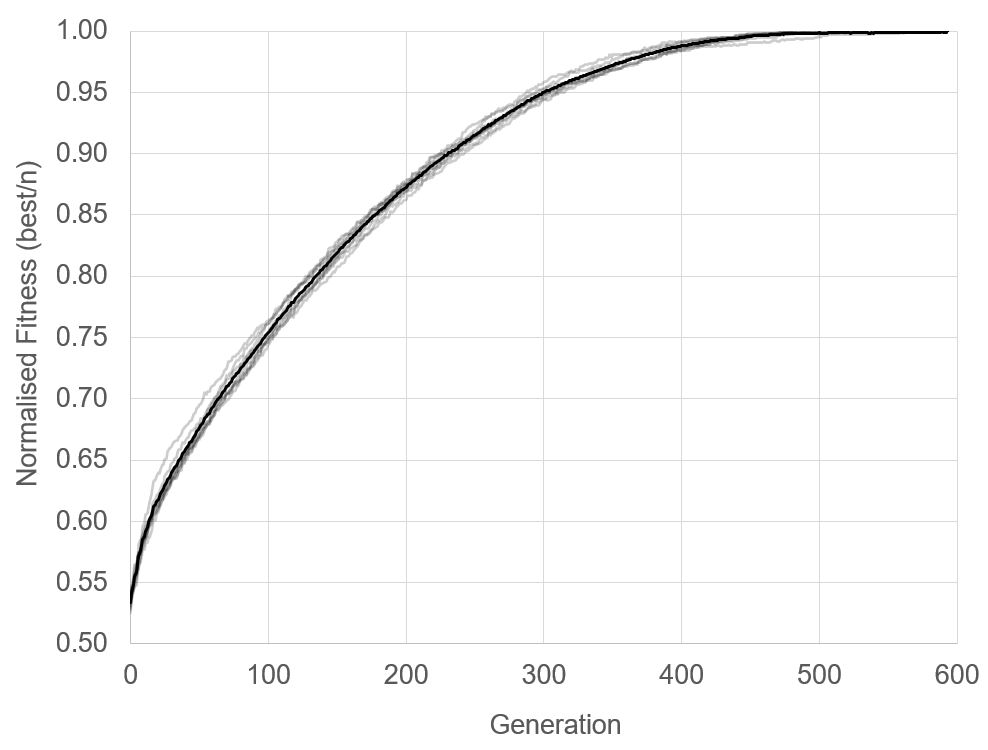
\includegraphics[scale=0.6]{normfit.png}
\caption{Normalised fitness vs number of generations, \(n\), for a population size of \(m=100\) and a chromosome size of \(n=1024\). Different random seeds where used (light grey results), with the average  plotted in black, demonstrating robust convergence for large problem size.}
\end{figure}

\newpage
\section{Performance Optimisation}

\subsection{Manual Optimisation}
An attempt was made to manually optimise the code based on gprof profiling. The program was compiled with the \textit{-pg -O0} flags set. Based on gprof profiling (see Annex B), the function \textit{Mutate} (see below), was identifed as taking approximately 21 percent of the runtime. 
\begin{lstlisting}
void Mutate(int *q, int n, int m)
{
    int mu;
    for (int i = 0; i < m; i++)
    {
        for (int j = 0; j < n; j++)
        {
            mu = (std::rand() % n);
            if (mu == 0)
            {
                (q(i, j)) = 1 - (q(i, j));
            }
        }

    }
    return;
}
\end{lstlisting}
An attempt was made to remove the internal branching as follows. 
\begin{lstlisting}
void Mutate(int *q, int n, int m)
{
    int mu;
    for (int i = 0; i < m; i++)
    {
        
        for (int j = 0; j < n; j++)
        {
            mu = ((std::rand() % n)==0);
            q(i, j) = (q(i, j))*(1-mu) + (1 - (q(i, j)))*(mu); //remove branching
        }

    }
    return;
}
\end{lstlisting}
However, followup profiling revealed that this actually made performance worse with the function \textit{Mutate} taking approximately 37 percent of the runtime. \cbstart On reflection, the likely reason the manual optimisation reduced performance was the additional calls to memory required for matrix \(q\). In the case that \(q\) is larger than the cache, the additional calls to memory to write values offset any advantage posed by reducing internal branching.  \cbend Therefore, this implementation was reverted and optimisation was focused on compile flags, as discussed in section 4.2


\subsection{Optimisation Flags}
Because of the number of nested loops in the \textit{Crossover}, \textit{Assess Individual fitness} and \textit{Mutate}, it was inferred that -funroll-loops would yield improvements.

What was unexpected, was the flags -flto and -fuse-linker-plugin in combination yielding a ~10-20 percent improvement on -O3 optimisation alone.  Although I do not  understand this improvement from the documentation, I hypothesise that these flags improve the optimization by exposing more code to the link-time optimizer. 

\subsection{Performance Results}
\label{serialperf}
\begin{figure}[H]
\centering
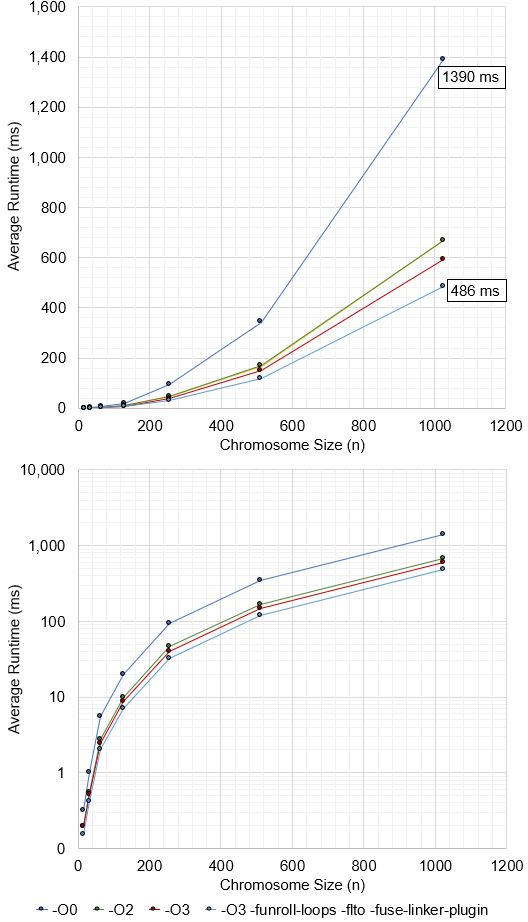
\includegraphics[scale=0.85]{avruntime2.png}
	\caption{Average runtime (ten trials) vs chromosome size, \(n\), for a population size of \(m=100\) individuals. Based on different optimisation flags a \(\sim 2.8\times\) speedup is achieved. These results were computed using the same random seed, \textit{seed }\(=42\).}
\end{figure}


\newpage
\chapter{Parallel Implementation}

\section{Parallelization Approach}

\subsection{Approach}
There are a large variety of ways to parallelize a GA, which are comprehensively discussed in \cite{nowostawski1999parallel}. To describe the parallel GA implementation in this work, the terminology in \cite{nowostawski1999parallel} has been adopted. 

The approach to parallelising the GA was to develop a number of \emph{static subpopulations with migration}. The population of individuals, \(m\), is divided into \emph{subpopulations} (also refereed to as \emph{demes}) of size \(m_{fraction}=m/k\), processed separately on \(k\) \emph{islands} that are \emph{geographically isolated}. In this model, a new operation, \emph{migration}, is added to the GA, which periodically exchanges individuals between islands (see Section \ref{Mig}).  

Reference \cite{nowostawski1999parallel} further categorises this parallelisation approach into \emph{coarse grained algorithms} and \emph{fine grained algorithms}.
Coarse grained algorithms have a relatively small number of demes with many individuals, periodically exchanged through migration. Fine grained algorithms divide the population into a larger number of small demes. Inter-deme communication is realised \emph{either} by using a migration operator, or by using overlapping demes.

For this work, MPI was used to parallellise the GA using a coarse grained approach. A coarse grained approach was selected because it allowed the majority of the original codebase developed in Chapter 1 to be reused\footnote{This was an important consideration because the serial GA implementation was verified to be working. A fine grained model would have required extensive revalidation of the \emph{crossover} and \emph{mutation} functions.}. Furthermore, it seemed to be the most directly comparable extension to the existing serial code. The parallel implementation 

\subsection{Migration}
\label{Mig}
Migration depends on several parameters such as the topology of the connections between the subpopulations, the number of individuals that migrate (i.e the \emph{migrants}), which individuals migrate and are replaced and the frequency of migration \cite{nowostawski1999parallel}. This work investigates the performance of two different migration topologies in addition to the number of \emph{migrants} as a percentage of the total population. Individuals are randomly selected for migration, with the array representing the migrating individual being copied (i.e. replacing) to the same individual in the subpopulation array at the destination island (per the movement of the coloured arrays in Figure \ref{migration_diagram} (b) and (c)). To limit the number of parameters requiring tuning, the \emph{migration interval} was set to one (i.e. migration is performed every generation). Given the communication overhead for parallelization, this selection is likely not optimal, especially for small problem sizes.

In addition to parallelization of the GA \emph{without} migration, this investigation explored two different migration strategies, referred to here as \emph{ring migration} and \emph{random migration}. These approaches are described with reference to Figure \ref{migration_diagram}. Without migration (Figure \ref{migration_diagram} (a)), the implementation is essentially a race between each of the islands to the fittest individual. An advantage of this approach is it's simplicity and low communication overhead, as the only inter-island communication is reporting the highest fitness achieved per generation. 

Ring migration (Figure \ref{migration_diagram} (b)) is one possible migration topology which is relatively simple to implement in MPI\footnote{This approach was inspired by the lecture series.}. Ring migration involves individuals migrating from island rank \(k\) to island rank \(k+1\), with the last individual migrating to island rank 0. Although simple to implement, this topology is not biologically/geographically inspired and is somewhat contrived.

\begin{figure}
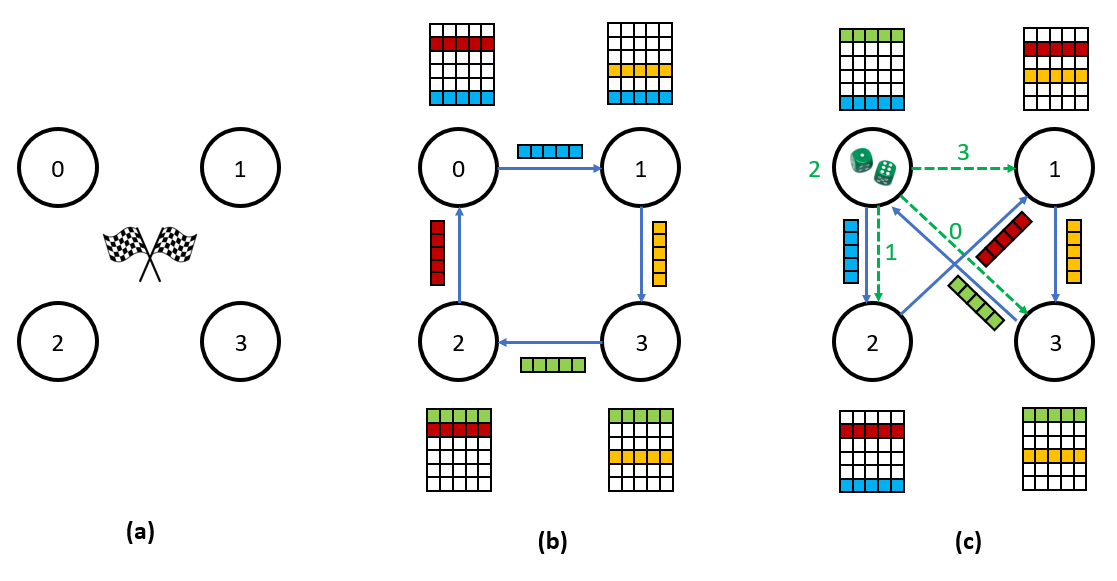
\includegraphics[scale=0.55]{migration_diagram}
\caption{Depiction of migration approaches investigated for \(k=4\) islands. Subfigure \textbf{(a)} depicts parallelisation \emph{without} migration, which is essentially a race to the maximum fitness individual between each of the subpopulations. Subfigures \textbf{(b)} and  \textbf{(c)} depicts ring migration and random migration, respectively. The blue arrows in subfigures \textbf{(b)} and  \textbf{(c)} represent the direction individuals migrate between islands in a generation. The green dashed arrows and numbers in subfigure \textbf{(c)} represents the random target islands (ranks) broadcast by island 0 to all islands, each generation.}
\label{migration_diagram}
\end{figure}

Random migration (Figure \ref{migration_diagram} (c)) involves migration from each island to a destination island of a random rank. MPI is based on all ranks having a deterministic set of communication patterns. As such, random communication patterns are somewhat more involved to implement in MPI. Each individual process uses a different random seed, to ensure the generation of distinct subpopulations. However, this means that if each individual process calls \texttt{std::rand()} independently to determine a random rank for migration, the processes will not know which island rank to receive communication (i.e. the island they receive migrants from). This implementation averts this difficulty by broadcasting an array of random integers, \emph{rand\_rank}, of length \emph{worldsize} from island rank 0 to all islands. The random communication can then be achieved by looping through the \(k\) islands, with island \(k\) sending and island \(rand\_rank[k]\) receiving. The array \(rand\_rank[k]\) is updated and broadcast each generation.


\section{Experimental Methodology and Plan}
\subsection{Overview}
The experiments planned for this investigation are separated into two parts. Firstly, a study will be made to determine which migration strategy (see Section \ref{Mig}) is best for the parallel implementation. The results of the migration experiments will inform the migration strategy for the larger scale performance experiments. The performance experiments will compare the performance of the serial and parallel algorithms for a variety of island numbers and chromosome sizes.  These experiments are detailed in Sections \ref{migexp} and \ref{perfexp}, respectively.
\subsection{Migration Experiments}
\label{migexp}
Rather than studying the optimality of migration for different problem scales, the objective of the migration investigation is to determine the (likely) best migration strategy to use for the performance experiments. The aim of the migration experiments is to determine 1) whether no migration, ring migration or rand migration offers the best performance and 2) to establish a number of migrants that provides robust performance, as a percentage of the total population. 

To limit the scope of this investigation, the migration results are obtained for a fixed \(n=1024\), \(m=128\), and \(k=4\). For each experiment, five trials were performed with different random seeds (see also discussion at Section \ref{perfexp}). The number of migrants was varied from 0 (no migration), 1, 5, 10, 16 and 32. The parameters for each of the migration experiments are specified in Table \ref{migtab}, below.
\begin{table}[h]
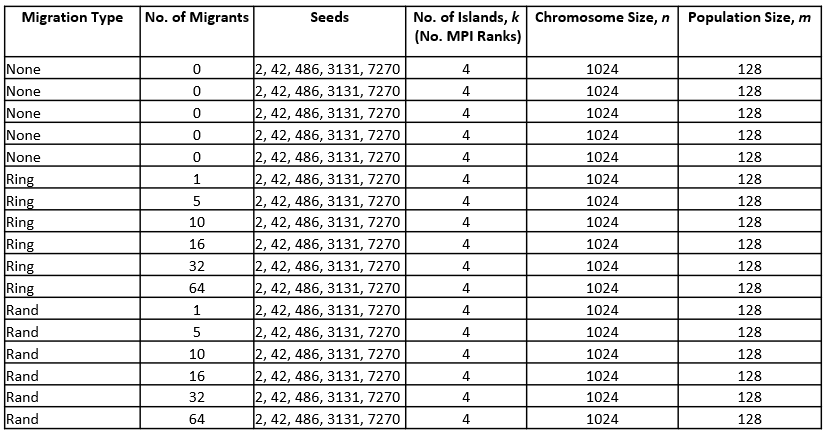
\includegraphics[scale=0.76]{migration_experiments}
\caption{Migration experiment parameters.}\label{migtab}
\end{table}

\subsection{Performance Experiments}
\label{perfexp}
The aim of the performance experiments is to determine how the runtime, \(T\), varies with chromosome size, \(n\), for a number of \emph{worldsizes} (i.e. no. islands, equivalent to MPI rank). The objective is to compare the scaling of the parallel implementation with the serial implementation, and to determine the respective empirical complexities.

Based on the results of the migration experiments, it was determined that random migration with a single migrant performed best for population size \(m\) (see migration  results in Section \ref{migresults}). Informed by these results, the performance experiments are conducted using random migration for a fixed population size, \(m=128\), and a fixed number of migrants, \(migrants=1\), with the chromosome size varying from \(n=16\) to \(n=32768\) and the number of islands varying from \(k=1\) (serial) to \(k=16\).

Over the course of development it was noticed that the variation in runtime of individual instances with the same random seed tended to be less than the variation due to runs with different random seeds. Therefore, it was decided that varying the random seed better captured the variation in output results possible with the GA than the ten repetitions with the same random seed performed for the serial implementation (see Section \ref{serialperf}). Therefore, for each performance experiment five trials are performed with the random seeds 2, 42, 486, 3131 and 7280.

The parameters for each of the performance experiments are specified in Table \ref{perftab}.


\subsection{Use of Stream Editor (sed)}
To automate the submission of jobs to the \texttt{getafix} cluster a bash script was developed to vary the input parameters. Because the program was structured to use macros for user defined constants (see Section \ref{progimp}), changing user parameters required \texttt{main.cpp} to be edited and the program recompiled. To enable this process to be automated using bash the stream editor (sed) was used in conjunction with regular expressions (regex). The stream editor can perform basic text transformations on an input stream, such as files. The following sed commands were used extensively to modify migration status, number of migrants, random seed and chromosome size. 
\begin{lstlisting}[language=bash]
sed -i '22 s/#define migration true/#define migration false/' main.cpp
sed -i "23 s/#define migrants [0-9]\+/#define migrants ${migrants}/" main.cpp
sed -i "17 s/#define seed [0-9]\+/#define seed ${seed}/" main.cpp
\end{lstlisting}
The stream editor was also used to modify the \texttt{goslurm.sh} slurm submission script for different numbers of islands, as follows
\begin{lstlisting}[language=bash]
sed -i "5 s/#SBATCH --ntasks=[0-9]\+/#SBATCH --ntasks=${islands}/" goslurm.sh
sed -i "6 s/#SBATCH --ntasks-per-node=[0-9]\+/#SBATCH --ntasks-per-node=${islands}/" goslurm.sh
\end{lstlisting}

The use of sed allowed the large number of performance experiments to be automatically compiled and submitted, without requiring the GA implementation to be modified to parse additional command line arguments. This reduced the likelihood of human error, a significant possibility given upwards of 240 compilations were required for the performance experiments alone\footnote{It was also quite satisfying.}.

\begin{table}[H]
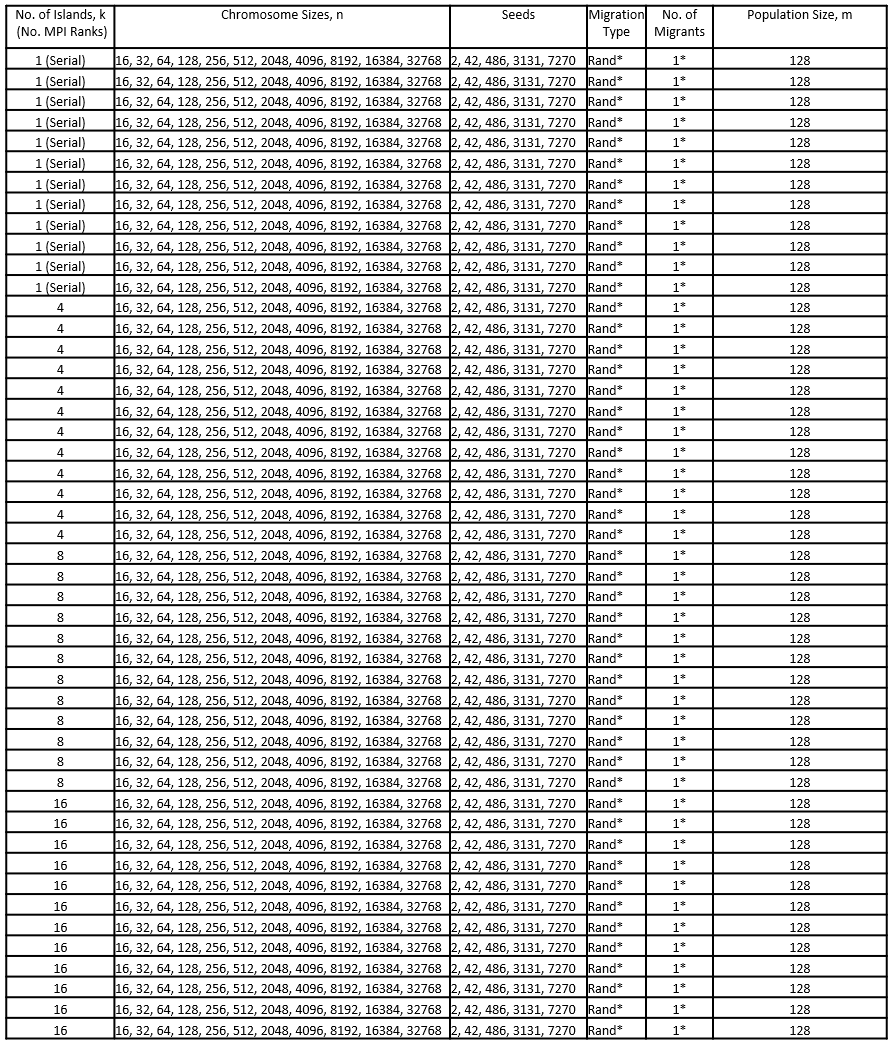
\includegraphics[scale=0.71]{performance_experiments}
\caption{Performance experiment parameters. The * denotes parameters which were selected based on the results of the migration experiments presented in Section \ref{migresults}.}\label{perftab}
\end{table}
\section{Results}
\subsection{Migration Results}
The migration results are plotted in Figure \ref{migresfig}. Figure \ref{migresfig} (a) clearly demonstrates that ring migration offers no benefit over no migration (i.e. migrant percentage of zero)), with runtime increasing approximately linearly with migrant percentage. However, Figure \ref{migresfig} (b) clearly demonstrates that for low migrant percentages of approximately 1-5 percent, random migration offers approximately a 30-35 percent improvement in runtime.

\label{migresults}
\begin{figure}[h]
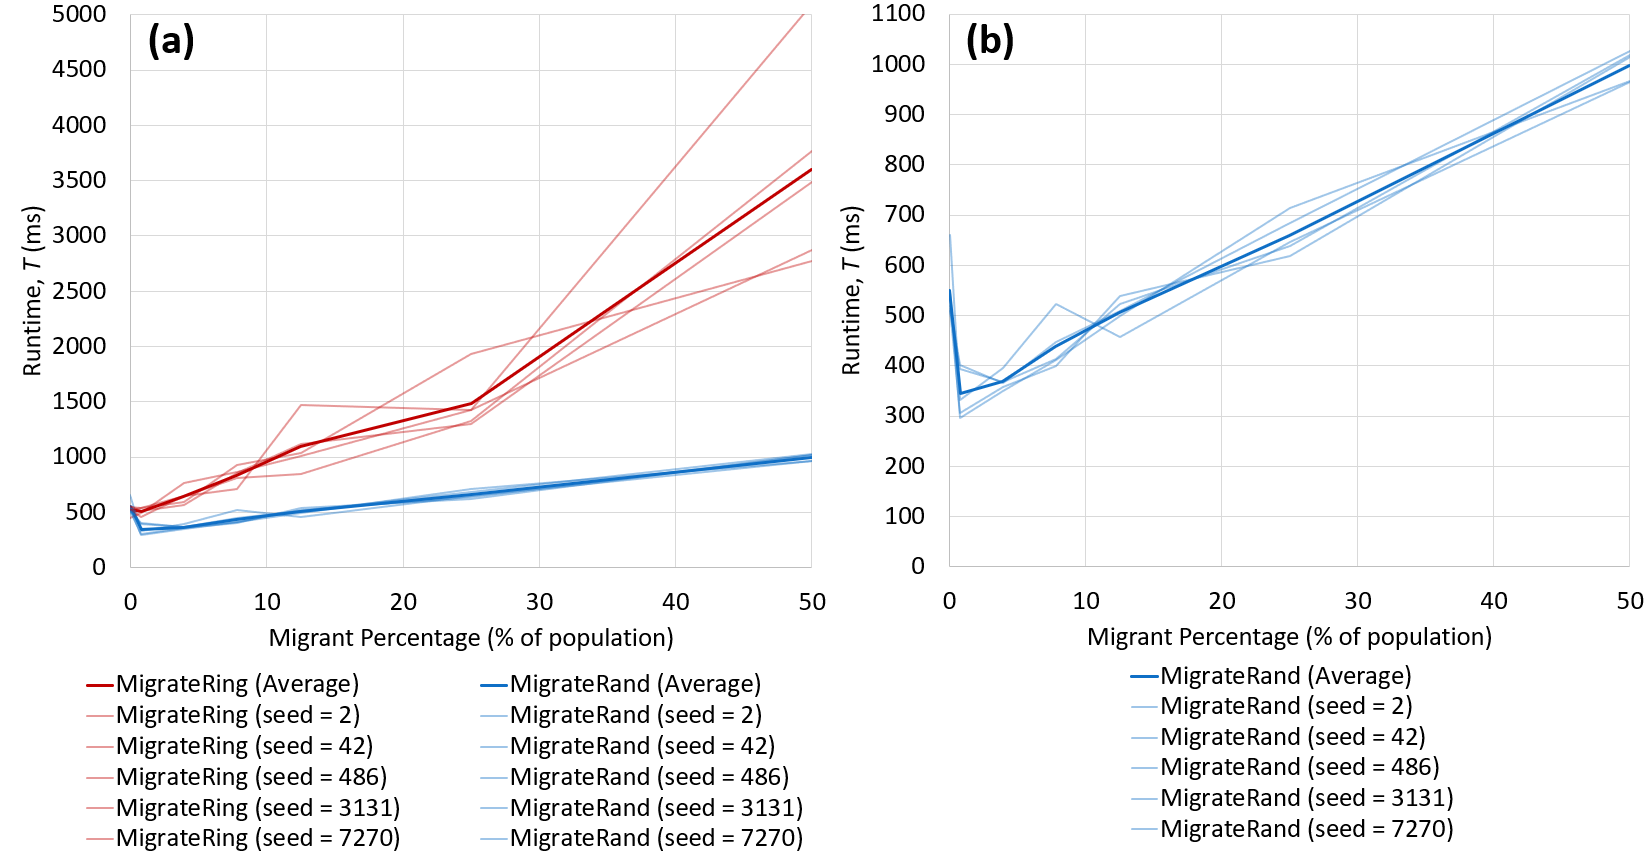
\includegraphics[scale=0.38]{migration_performance}
\caption{Migration results for both ring migration and random migration are presented in subfigure \textbf{(a)}. Subfigure \textbf{(b)} zooms in on the random migration results.}\label{migresfig}
\end{figure}

\subsection{Performance Results}
The runtime as a function of chromosome size is plotted in Figure \ref{runtimeperf}. Figure \ref{runtimeperf} clearly demonstrates performance improvements for increasing numbers of islands. Figure \ref{runtimeperf} also demonstrates that the variance in runtime associated with the different random seeds is significantly lower for the 16 island experiment, compared with the other experiments.  


As discussed by Coffin and Saltzman in \cite{coffin2000statistical}, if we parametrise the runtime, \(T\), by the chromosome size, \(n\), as 
\begin{align*}
T(n) = Cn^k,
\end{align*}
where \(C\) and \(k\) are regression parameters. By taking a regression of the log-transformed model, the gradient estimates the algorithm's order of the computational complexity, \(O(n^k)\), the \textit{empirical complexity},
\begin{align*}
\ln T(n) = \ln C + k \ln n.
\end{align*}

A log regression is performed for the serial results in Figure \ref{logruntimeperf}. The log regression gradient of approximately 2 indicates the empirical complexity of the serial GA is \(O(n^2)\).  The parallel GA tents towards the same gradient for increasing \(n\), indicating the \(O(n^2)\) complexity holds in the limit of large \(n\). 

Figure \ref{logruntimeperf} also demonstrates that for small \(n\) the parallel GA performs significantly worse than the serial implementation, due to the communications overhead required to initialise all islands, and check global fitness. This is only apparent in the log scaling of Figure \ref{logruntimeperf}. 

Figure \ref{speedup} demonstrates the average runtime speedup of the parallel GA relative to the serial GA as a function of the number islands for different chromosome sizes \(n\). As with Figure \ref{logruntimeperf}, we observe that the parallel GA reduces the performance for small problem sizes \(n=64,256\). Conversely, for the large problem sizes \(n=8192, 32768\), The speedup approaches the limit of linear scaling with additional CPUs. For example, the maximum speedup achieved for 

\begin{figure}[h]
\centering
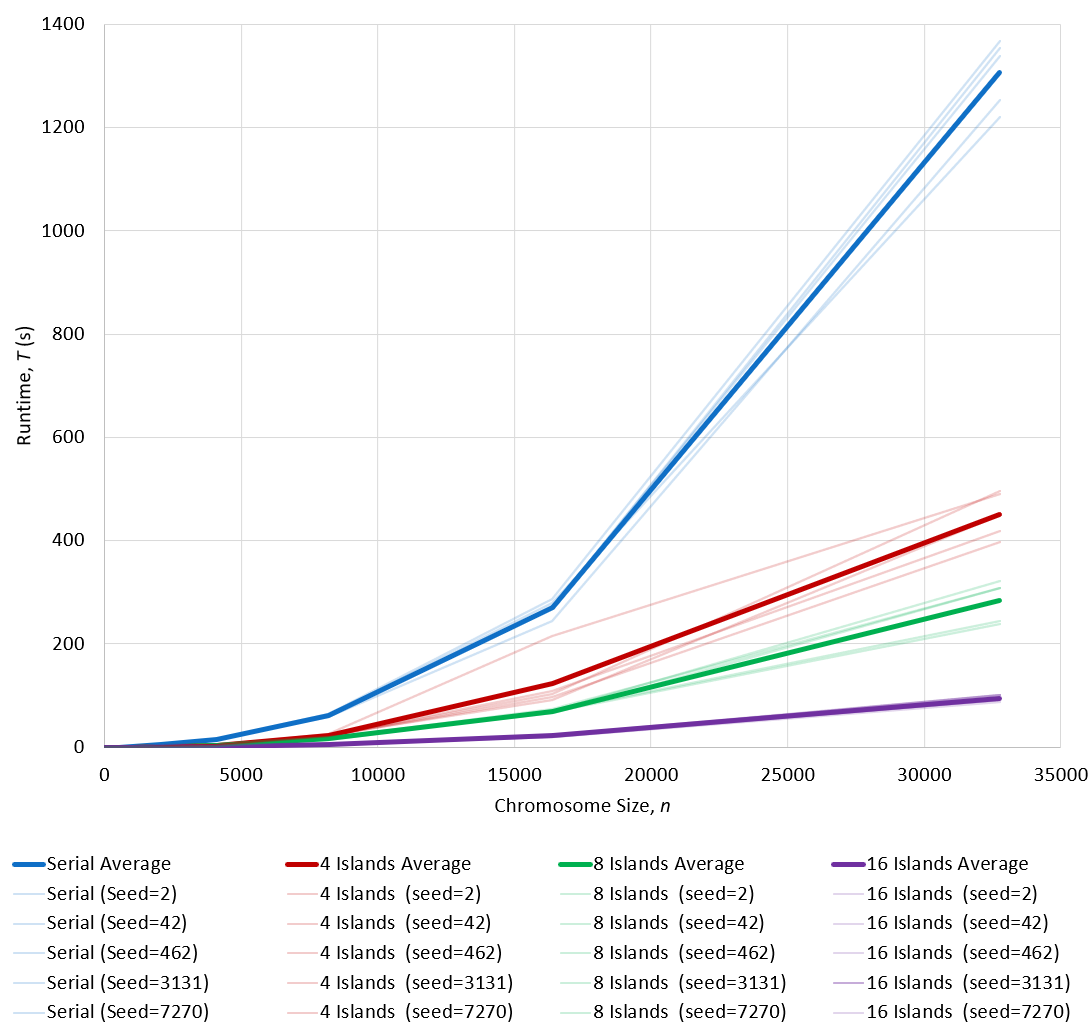
\includegraphics[scale=0.4]{runtime_perf}
\caption{Runtime as a function of chromosome size for different numbers of islands (MPI ranks).}\label{runtimeperf}
\end{figure}
\begin{figure}[H]
\centering
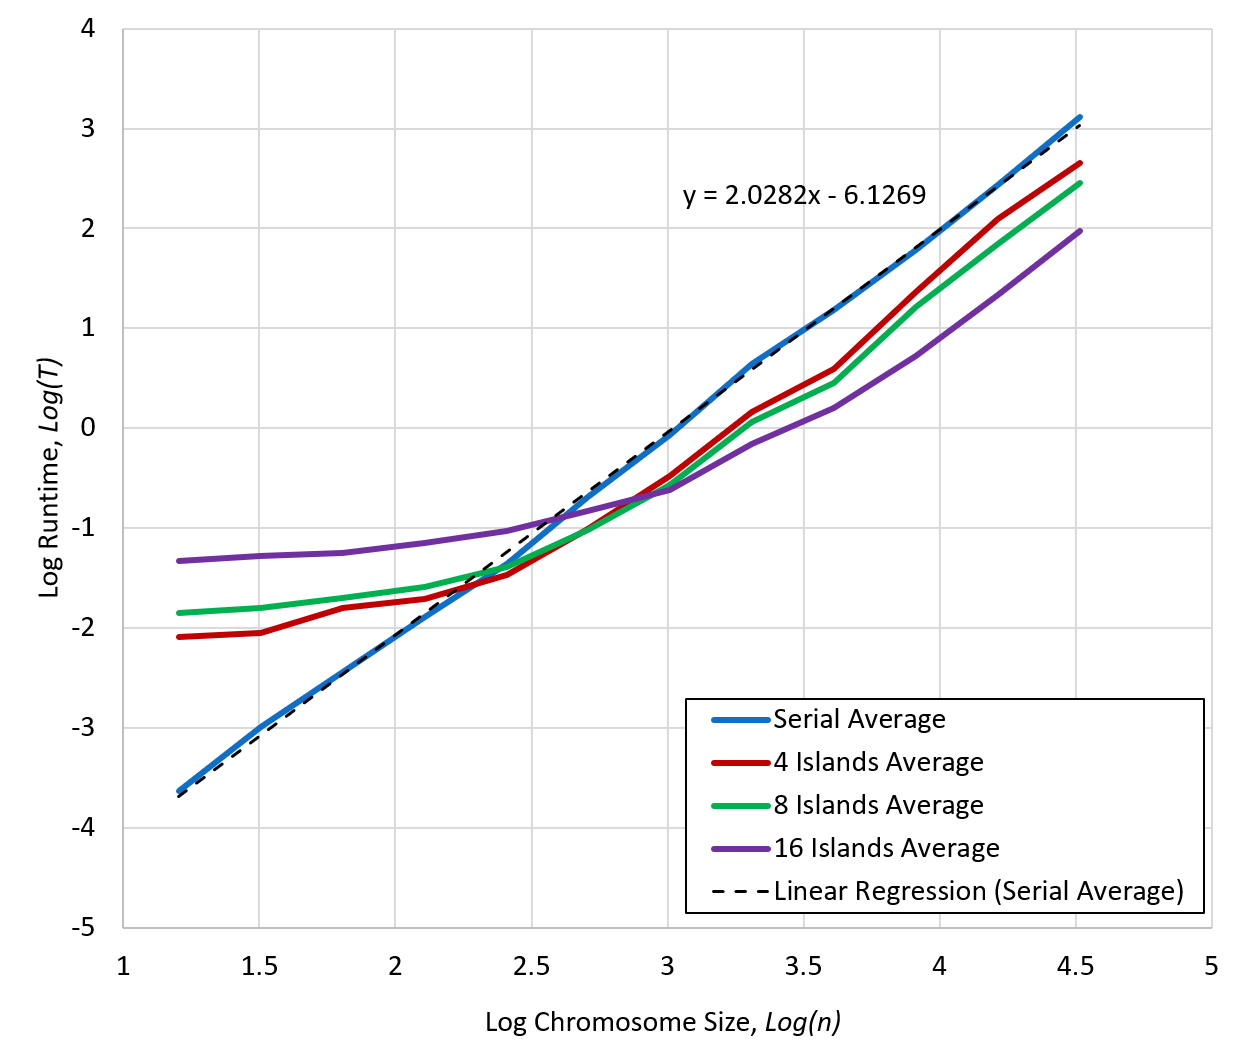
\includegraphics[scale=0.385]{logruntime_perf}
\caption{Log runtime as a function of log chromosome size for different numbers of islands (MPI ranks). A linear regression of the serial results is included with the equation depicted on the plot. }\label{logruntimeperf}
\end{figure}

\begin{figure}[H]
\centering
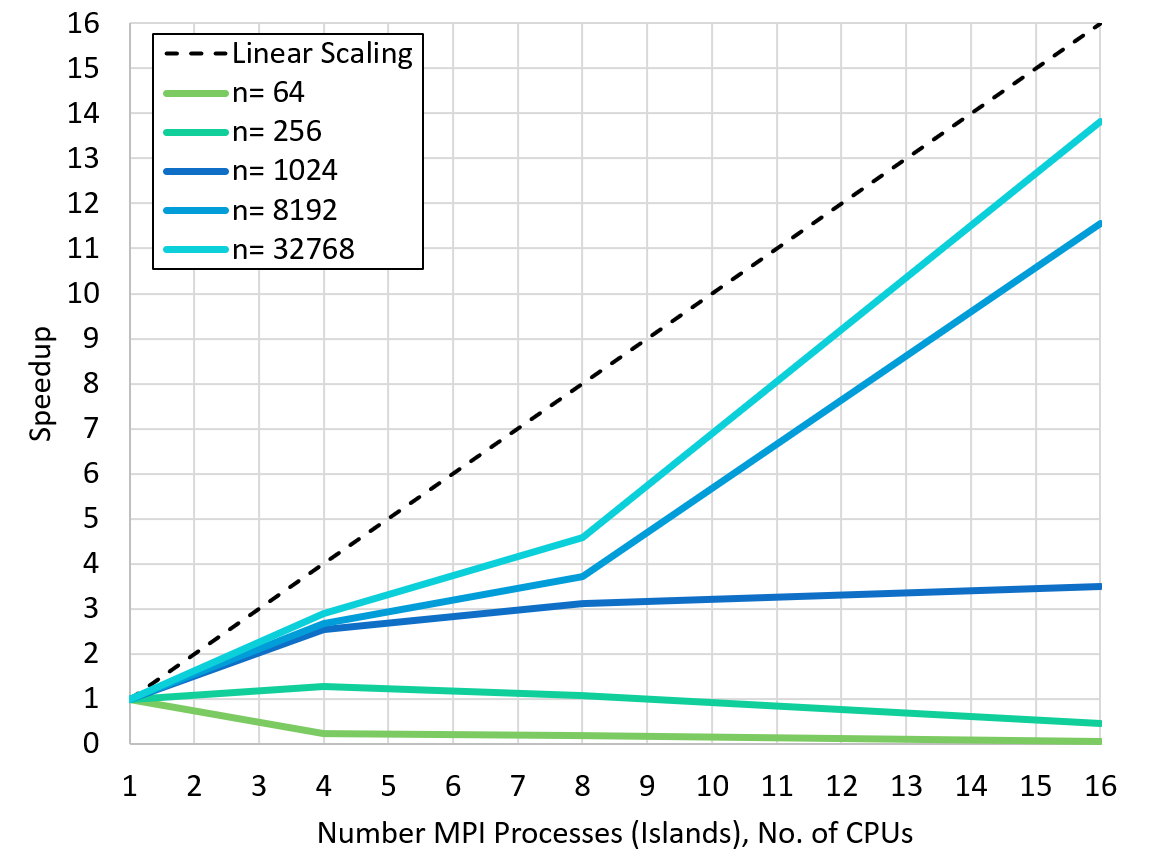
\includegraphics[scale=0.385]{speedup}
\caption{Average runtime speedup as a function of number of islands (MPI ranks) for chromosome sizes from \(n=64\) to \(n=32768\).}\label{speedup}
\end{figure}





\section{Discussion}
\subsection{Outcomes}
One of the main findings of this investigation was the superior performance of random migration compared with ring migration. Superficially, this result is somewhat unexpected as the random migration involves and additional  MPI broadcast call to distribute \emph{rand\_rank} in addition to the send and receive calls conveying the migrating individuals. However, the improvement in convergence rate was observed to more than make up for the additional broadcast call.  

Somewhat imprecisely, this can be explained by considering the spread of successful individuals throughout the world. If there is a successful individual on an island through selection and crossover its genes become more prevalent in that population. Therefore, an individual containing at least some of these  successful genes is more likely to be randomly selected for migration. In ring migration, these successful genes only travel to an adjacent island, where they must build up a majority to be likely to migrate to the next adjacent island. In random migration, successful genes are sent to an island of random rank, each generation, rather than incrementally populating their way through the loop. With this explanation in mind, it would be interesting to test the two migration strategies on a problem other than OneMax, with more local optima\footnote{Such as the Rastrigin, Schwefel or Griewank problems in \cite{Luke2013Metaheuristics}}. In this scenario, random migration may favour the propagation of local optima, reducing the diversity required to reach the global optima.

Another finding is that migration only yields an improvement for low migrant numbers, between 1 and 5 percent of the global population. This is understood in the context of the afore explanation, to be due to the penalty of communications overhead. Since more successful solutions tend to be more prevalent throughout a subpopulation at any time, repeated random sampling and propagating yields diminishing returns as similar genes are likely to be propagated, offering little convergence advantage with the same communications overhead. 

The the performance experiments were successful in determining 

\subsection{Limitations}
Only works for combinations of population size and number of islands that are evenly divisible. 

SIngle point vs double point crossover

Other implementations incorporate a version of \emph{elitism} for the migration step.\cite{muhlenbein1991parallel}
The migration step may occur less frequently than every iteration - this was not studied.
More complex migration topologies, such as nearest neighbour, were not explored.
The migration interval of one was not optimal, especially for small problem sizes, due to the communcations overhead.
Parallel GAs have many control parameters - difficult to devise (efficient) experiments to optimise performance. Somewhat an art.
Drawbacks of  \texttt{std::rand()}
\newpage

\section{Conclusion}
This work successfully demonstrated the performance scaling of a parallel GA for the OneMax problem, using  islands of subpopulations with migration. The final implementation was informed by a parameter and algorithm study, which determined that random migration of 1-5 percent of the population provided the best performance. 

Empirical time complexity of the serial GA was estimated to be \(O(n^2)\) using log regression.  The parallel GA tents towards the same gradient for increasing \(n\), indicating the \(O(n^2)\) complexity holds in the limit of large \(n\). 
 
\bibliographystyle{ieeetr}
\bibliography{coscbibdemo}

\newpage

\chapter*{Annexes}


\section*{Annex A - Serial Verbose Example}
Using the following inputs, the verbose output for a single loop is displayed as an example.
\begin{lstlisting}
#define n 16                  // Chromosome size (number of genes per individual).
#define m 8                   // Population size (number of individuals).
#define seed 42               // Psuedorandom number generator seed (std:srand(seed)).
#define maxgenerations 2000   // Maximum number of generations (while loop limit).
#define t 2                   // Tournament size (parents competing for selection).
#define verbose true          // Verbose output (cout) for verification.
#define printfitness false    // Best fitness per generation output (cout).
\end{lstlisting}
Single loop (generation) verbose output (cout):
\begin{lstlisting}
Running MaxFitness (Verbose)
0011001011011000 -> Individual 0, Fitness: 7
0001101111101011 -> Individual 1, Fitness: 10
0000011011101111 -> Individual 2, Fitness: 9
0101010111101110 -> Individual 3, Fitness: 10
1100010101010110 -> Individual 4, Fitness: 8
0110111001000101 -> Individual 5, Fitness: 8
0010010000011111 -> Individual 6, Fitness: 7
0101011101100100 -> Individual 7, Fitness: 8
 ------------ Generation: 0 Best Fitness: 10 --------------
Running Crossover (Verbose)
Crossover at chromosome 7:
0001101|111101011 -> Parent 1 (Individual 1)
0110111|001000101 -> Parent 2 (Individual 5)
0001101|001000101 -> Child 0
0110111|111101011 -> Child 1
Crossover at chromosome 7:
0110111|001000101 -> Parent 1 (Individual 5)
1100010|101010110 -> Parent 2 (Individual 4)
0110111|101010110 -> Child 2
1100010|101000101 -> Child 3
Crossover at chromosome 15:
000110111110101|1 -> Parent 1 (Individual 1)
010101011110111|0 -> Parent 2 (Individual 3)
000110111110101|0 -> Child 4
010101011110111|1 -> Child 5
Crossover at chromosome 0:
|0001101111101011 -> Parent 1 (Individual 1)
|0001101111101011 -> Parent 2 (Individual 1)
|0001101111101011 -> Child 6
|0001101111101011 -> Child 7
Running Mutate (Verbose)
 0  0  0  1  1  0  1 *1* 0  1  0  0  0 *0* 0  1 -> Child 0 Mutation at *_* 
 0  1  1  0  1  1  1  1  1  1  1  0  1  0  1  1 
 0  1  1  0  1  1  1  1 *1* 1  0  1  0  1  1  0 -> Child 2 Mutation at *_* 
 1 *0* 0  0  0  1  0  0  0  1 *1* 0  0  1  0  1 -> Child 3 Mutation at *_* 
 0  0  0  1  1  0 *0* 1  1  1  1  0  1  0  1  0 -> Child 4 Mutation at *_* 
 0  1  0  1  0  1  0  1  1  1  1  0  1  1  1  1 
 0  0  0  1  1  0  1  1  1  1  1  0  1  0  1  1 
 0  0  0  1  1  0  1  1  1  1  1  0  1  0  1  1 
Assigning next generation (Verbose)
0001101101000001 -> Child 0 to Individual 0, Fitness: 6
0110111111101011 -> Child 1 to Individual 1, Fitness: 12
0110111111010110 -> Child 2 to Individual 2, Fitness: 11
1000010001100101 -> Child 3 to Individual 3, Fitness: 6
0001100111101010 -> Child 4 to Individual 4, Fitness: 8
0101010111101111 -> Child 5 to Individual 5, Fitness: 11
0001101111101011 -> Child 6 to Individual 6, Fitness: 10
0001101111101011 -> Child 7 to Individual 7, Fitness: 10
\end{lstlisting}

\newpage
\section*{Annex B - Serial Profiling Results}

Initial gprof results, prior to (attempted) manual optimisation of the function \textit{Mutate}.
\begin{lstlisting}
Each sample counts as 0.01 seconds.
  %   cumulative   self              self     total           
 time   seconds   seconds    calls  ms/call  ms/call  name    
 38.19      0.45     0.45   144600     0.00     0.00  IndividualFitness(int, int*, int, int)
 21.21      0.70     0.25      482     0.52     0.52  Mutate(int*, int, int)
 17.82      0.91     0.21      482     0.44     0.44  NextGeneration(int*, int*, int, int)
 11.88      1.05     0.14      483     0.29     0.29  MaxFitness(int*, int, int)
 10.18      1.17     0.12      482     0.25     1.20  Crossover(int, int*, int*, int, int)
  0.85      1.18     0.01    48200     0.00     0.01  TournamentSelection(int, int*, int, int)
  0.00      1.18     0.00        1     0.00     0.00  _GLOBAL__sub_I__Z14ParseArgumentsiPPc
  0.00      1.18     0.00        1     0.00     0.00  _GLOBAL__sub_I_useseed
  0.00      1.18     0.00        1     0.00     0.00  PrintFitness(int*, int)
  0.00      1.18     0.00        1     0.00     0.00  RandomPopulation(int*, int, int)
  0.00      1.18     0.00        1     0.00     0.00  __static_initialization_and_destruction_0(int, int)
  0.00      1.18     0.00        1     0.00     0.00  __static_initialization_and_destruction_0(int, int)
\end{lstlisting}
gprof results, after to (attempted) manual optimisation of the function \textit{Mutate}. Subsequently, the initial implmentation of mutate was used. 
\begin{lstlisting}
Each sample counts as 0.01 seconds.
  %   cumulative   self              self     total           
 time   seconds   seconds    calls  ms/call  ms/call  name    
 37.98      0.55     0.55      482     1.14     1.14  Mutate(int*, int, int)
 27.62      0.95     0.40   144600     0.00     0.00  IndividualFitness(int, int*, int, int)
 12.43      1.13     0.18      482     0.37     1.20  Crossover(int, int*, int*, int, int)
 10.36      1.28     0.15      483     0.31     0.31  MaxFitness(int*, int, int)
  8.98      1.41     0.13      482     0.27     0.27  NextGeneration(int*, int*, int, int)
  0.00      1.41     0.00    48200     0.00     0.01  TournamentSelection(int, int*, int, int)
  0.00      1.41     0.00        1     0.00     0.00  _GLOBAL__sub_I__Z14ParseArgumentsiPPc
  0.00      1.41     0.00        1     0.00     0.00  _GLOBAL__sub_I_useseed
  0.00      1.41     0.00        1     0.00     0.00  PrintFitness(int*, int)
  0.00      1.41     0.00        1     0.00     0.00  RandomPopulation(int*, int, int)
  0.00      1.41     0.00        1     0.00     0.00  __static_initialization_and_destruction_0(int, int)
  0.00      1.41     0.00        1     0.00     0.00  __static_initialization_and_destruction_0(int, int)
\end{lstlisting}

\newpage
\section*{Annex C - Shell Scripts to Automate slurm Submission}
\begin{lstlisting}[language=bash]
islands=$1
migrants=1

sed -i "5 s/#SBATCH --ntasks=[0-9]\+/#SBATCH --ntasks=${islands}/" goslurm.sh
sed -i "6 s/#SBATCH --ntasks-per-node=[0-9]\+/#SBATCH --ntasks-per-node=${islands}/" goslurm.sh

#2048 4036 8192 16384 32768
#16 32 64 128 256 512 1024

for seed in 42 3131 462 2 7270
do
    for sizen in 16 32 64 128 256 512 1024
    do
        outputname="Parallel_${migrants}_${sizen}_${seed}_${islands}"
        echo ${outputname}
        sed -i "3 s/#SBATCH --job-name=\(.*\)/#SBATCH --job-name=${outputname}/" goslurm.sh
        sed -i "17 s/#define seed [0-9]\+/#define seed ${seed}/" main.cpp
        sed -i "15 s/#define n [0-9]\+/#define n ${sizen}/" main.cpp
        if [ $migrants -eq 0 ]
        then 
            sed -i '22 s/#define migration true/#define migration false/' main.cpp
            sed -i "23 s/#define migrants [0-9]\+/#define migrants ${migrants}/" main.cpp
        else
            sed -i '22 s/#define migration false/#define migration true/' main.cpp 
            sed -i "23 s/#define migrants [0-9]\+/#define migrants ${migrants}/" main.cpp 
        fi
       mpic++ -std=c++11 -g -O3 -funroll-loops -flto -fuse-linker-plugin functions.cpp main.cpp -o ${outputname}
       sleep 6
       sbatch goslurm.sh ${islands} 
       sleep 2
    done
done
\end{lstlisting}

\end{document}


\begin{lstlisting}
int** p = new int*[m];
for(int i = 0; i < m; ++i)
{
	p[i] = new int[n];
}
\end{lstlisting}


\begin{center}
\begin{tabular}{|l|cccc|}
\hline
Processors	&1		&2		&4		&8 \\
\hline
Runtime (s) 	&1400 &900  &600  &500\\
\hline
\end{tabular}
\end{center}

\begin{center}
\begin{figure}[h]
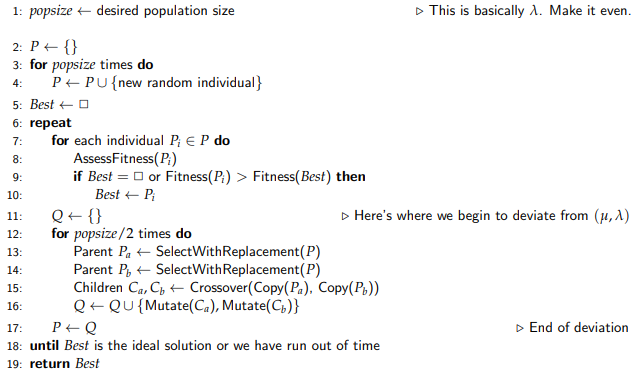
\includegraphics[scale=0.5]{genalg.png}
	\caption{Average runtime (ten trials) vs chromosome size, \(n\), for a population size of \(m=100\) individuals. Based on different optimisation flags a \(\sim 3\times\) speedup is achieved. These results were computed using the same random seed, \textit{seed }\(=42\).}
\end{figure}
\end{center}